\documentclass[aspectratio=169]{beamer} % 16:9 aspect ratio for modern screen
% \documentclass[handout]{beamer}
% \documentclass[notes=only]{beamer}

% Theme settings
\usetheme[progressbar=foot]{metropolis} % Minimalist theme
\metroset{progressbar=frametitle} % Progress bar soll nur folien mit titel berücksichtigtigen?
\setbeamercolor{background canvas}{bg=white} % White background color

\makeatletter
    \setlength{\metropolis@progressinheadfoot@linewidth}{1.5pt}
\makeatother


\usefonttheme{professionalfonts} % Font theme

% Packages
\usepackage[T1]{fontenc}   % Font encoding
\usepackage[ngerman]{babel} % German language
\usepackage[sfdefault]{FiraSans} % For FiraSans font
\usepackage[backend=biber, style=authoryear-comp
, sorting=nyt]{biblatex} % For bibliography
\usepackage{csquotes} % Recommended for biblatex with babel/polyglossia
\usepackage{textgreek} % Greek letters in text mode (aus references von Citavi)
\usepackage{tikz}          % For drawing graphics
\usepackage{animate} % Für Animation

\usepackage{graphicx}       % For including images
\usepackage{amsmath, amssymb} % For math symbol

% \usepackage{media9} % For embedding videos

\usepackage[labelformat=empty]{caption}


% Bibliography settings
\addbibresource{references.bib} % Path to the bibliography file

% Graphics path
\graphicspath{{Images/}} % Path to images folder

% custom Citation commands
\DeclareCiteCommand{\citeauthortitle}
  {\usebibmacro{prenote}}
  {\usebibmacro{citeindex}%
   \printnames{labelname}%
   \setunit{\space\textendash\space}
   \printfield{title}}
  {\multicitedelim}
  {\usebibmacro{postnote}}

  \DeclareCiteCommand{\citeauthortitleurl}
  {\usebibmacro{prenote}}
  {\usebibmacro{citeindex}%
   \printnames{labelname}%
   \setunit{\space\textendash\space}
   \printfield{title}%
   \setunit{\addsemicolon\space}
   \printfield{url}}
  {\multicitedelim}
  {\usebibmacro{postnote}}

\DeclareCiteCommand{\parenciteauthortitle}
  {\usebibmacro{prenote}}
  {\bibopenparen\usebibmacro{citeindex}%
   \printnames{labelname}%
   \setunit{\space\textendash\space}% <- Hier wird das Trennzeichen ":" hinzugefügt
   \printfield{title}\bibcloseparen}
  {\multicitedelim}
  {\usebibmacro{postnote}}

\makeatletter
\renewcommand\footnotesize{\tiny}
\makeatother

\newcommand{\figcite}[1]{\\[-3mm]{\tiny Quelle: \cite{#1}}}
\newcommand{\figciteweb}[1]{\\[-3mm]{\tiny aus: \citeauthortitle{#1}}}
\newcommand{\figciteweburl}[1]{\\[-3mm]{\tiny aus: \citeauthortitleurl{#1}}}
  
\mode<handout>{
    \AtBeginSection[]{} % In Handout-Version keine Section-Folie erzeugen
}

% Title page settings
\title{Space Radiation Effects in Electronics}
\subtitle{Weltraumstrahlungseffekte in der Elektronik}
\author{Florian Marius Adamczyk}
\date{\today}
\institute{Justus-Liebig-Universität Gießen \\ Modul \textbf{Wissenschaftliches Präsentieren} bei \\ \textbf{Prof. Dr. Derck Schlettwein, PD Dr. Daniel Ebeling, Dr. Ulrike Nespital}\\
Themavergabe und Betreuer: \textbf{Dr. Roman Bergert}}
\titlegraphic{\vspace{-1cm}\includegraphics[height=1.2cm]{Images/jlu_logo.jpg}}

\begin{document}

    Black slide, then introduction images:
    \begin{frame}<handout:0>[plain, noframenumbering]
      \begin{tikzpicture}[remember picture, overlay]
        % schwarzer Hintergrund (bleibt hinter den Bildern)
        \fill[black] (current page.south west) rectangle (current page.north east);
      \end{tikzpicture}
      \centering

      \only<1>{\includegraphics[height=\textheight]{Space_radiation_ESA.jpg}\\
      \tiny \textcolor{gray}{\citeauthor{10843774} -- \citetitle{10843774}}}

      \centering
      % Overlay 1: nur schwarz
      \only<2>{}

      % Overlay 2: erstes Bild über dem schwarzen Hintergrund
      \only<3>{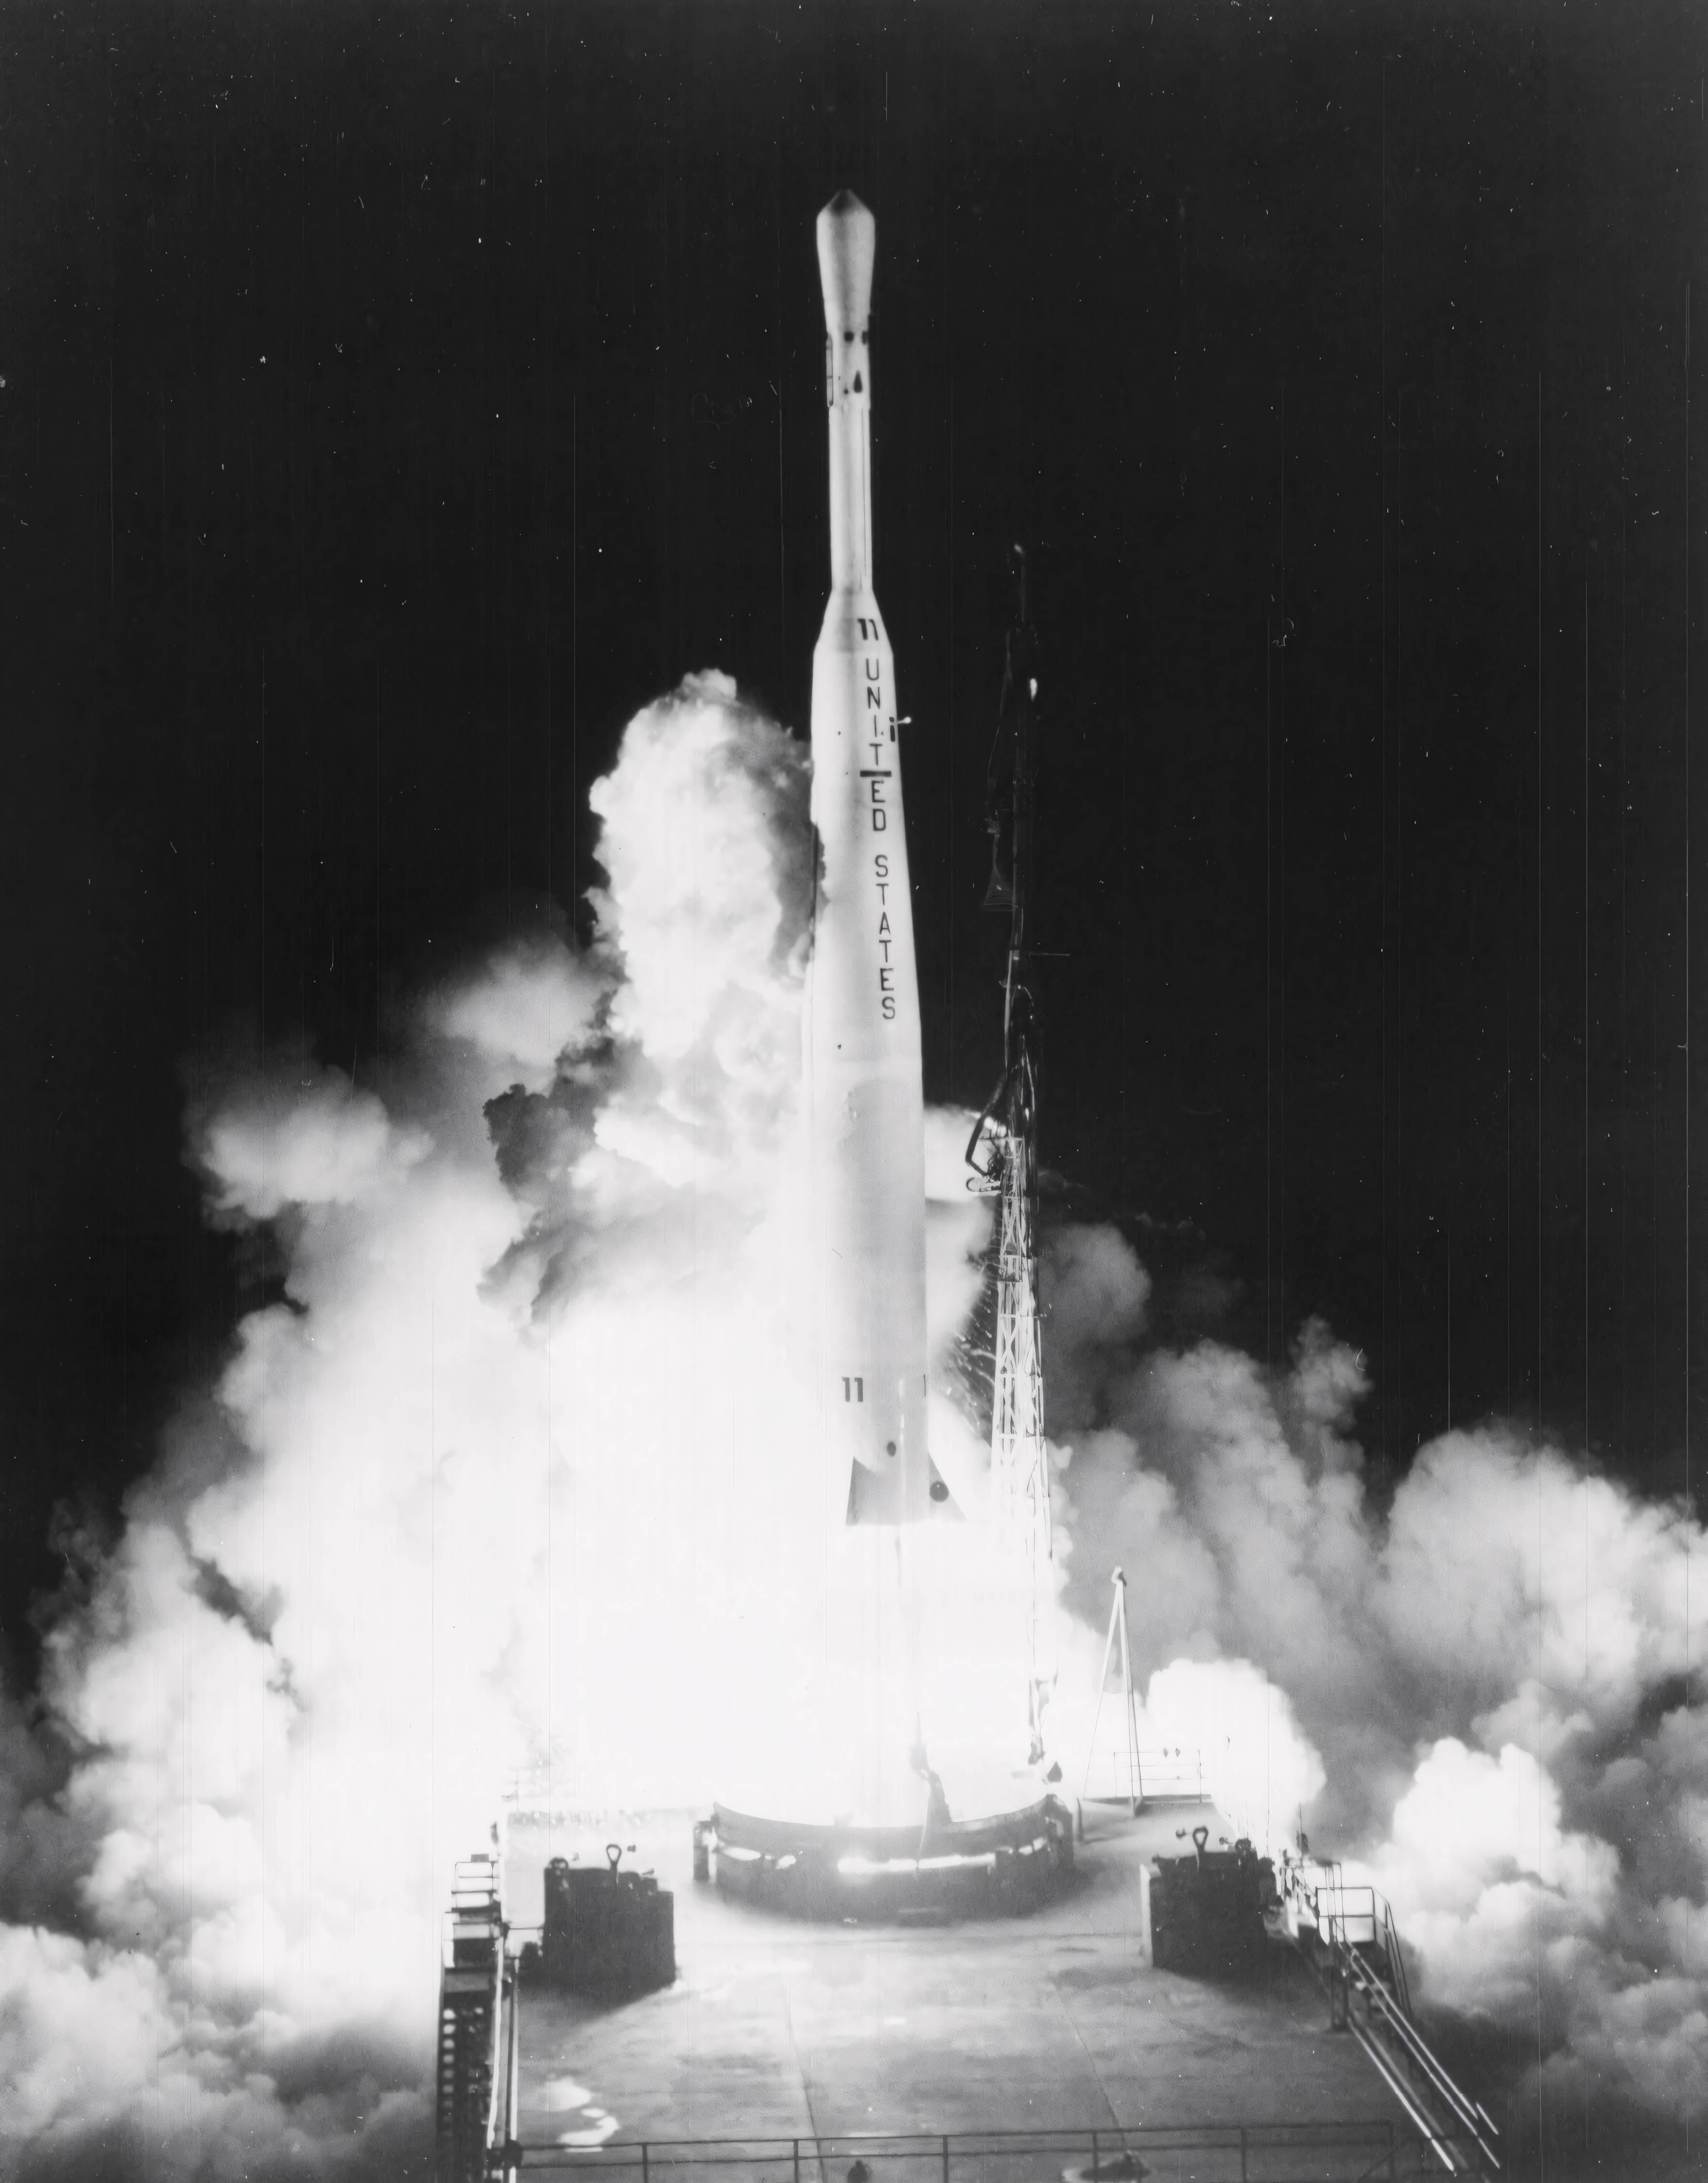
\includegraphics[height=\textheight]{Delta_Rocket_Telstar1_upscayl_2x_ultramix-balanced-4x.png}\\
      \tiny \textcolor{gray}{\citetitle{delta_rocket_telstar1_46898} -- \citefield{delta_rocket_telstar1_46898}{note}}}
      % Overlay 3: zweites Bild ersetzt das erste
      \only<4>{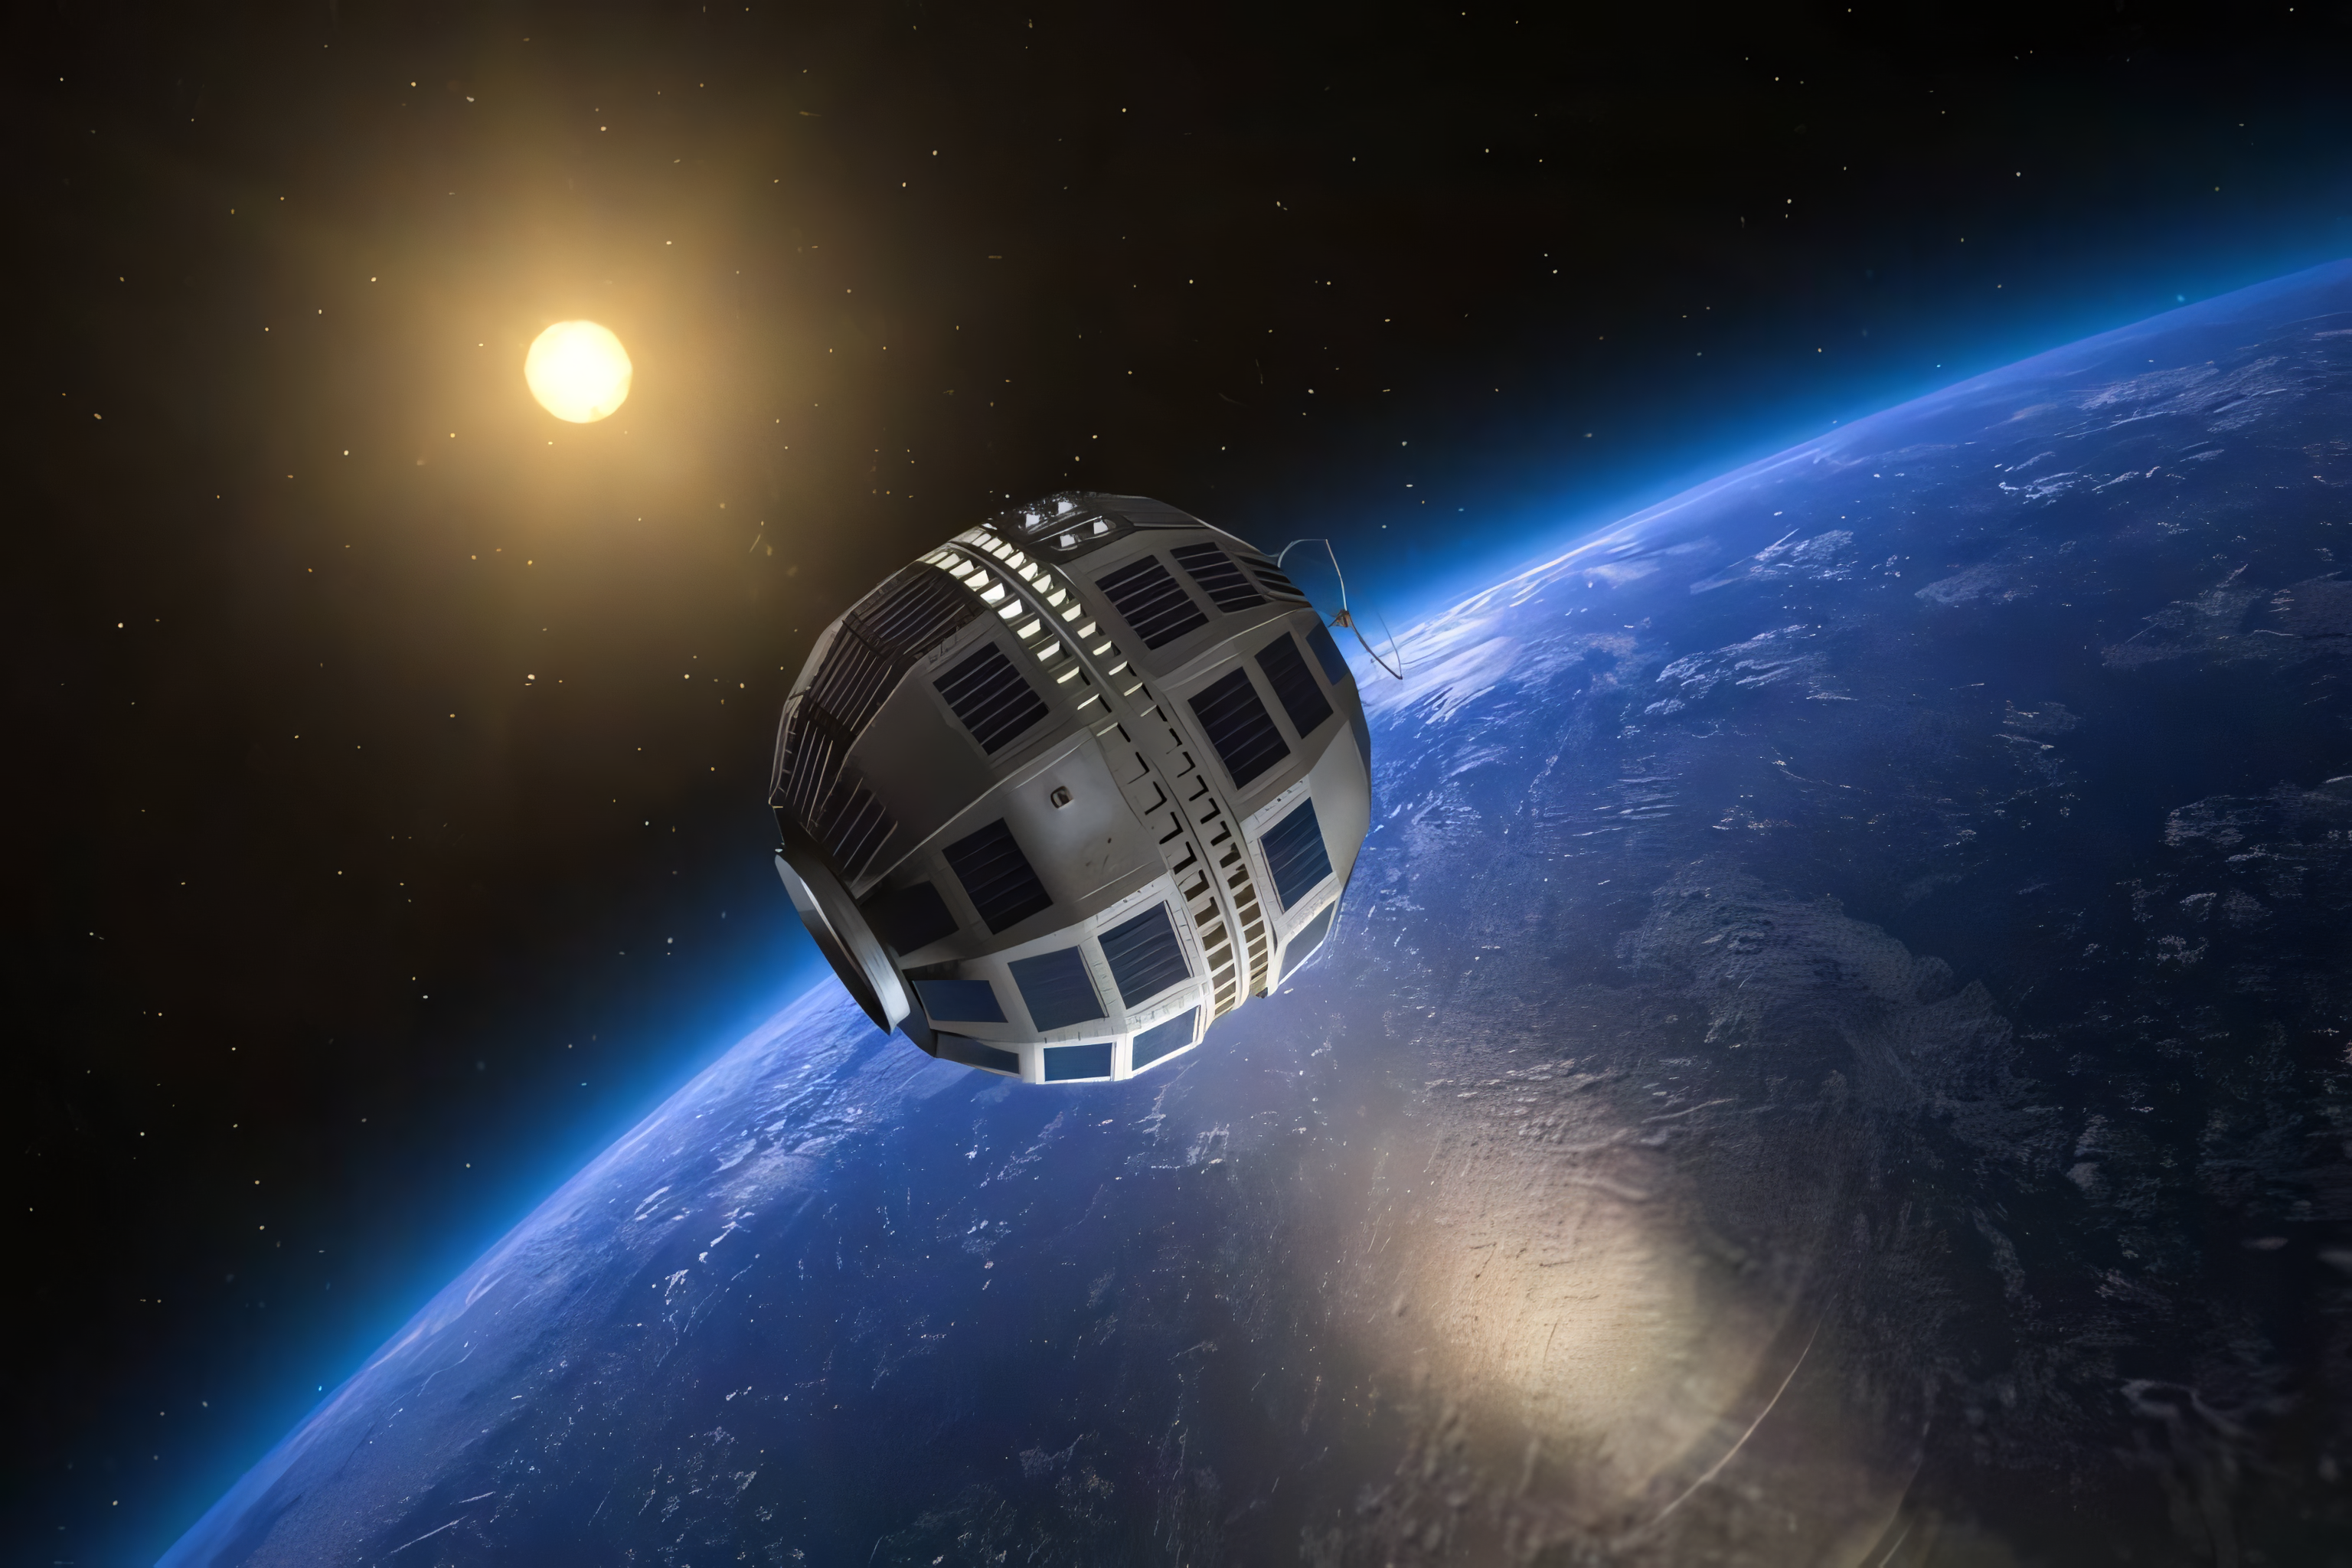
\includegraphics[height=\textheight]{Telstar1_upscayl_4x_ultramix-balanced-4x.png}\\
      \tiny \textcolor{gray}{\citeauthor{adobe_174965630_2025} -- \citefield{adobe_174965630_2025}{note}}}

      \only<5>{\includegraphics[height=\textheight]{p027c61m.jpg}\\
      \tiny \textcolor{gray}{\citeauthor{bbc_2024_first_live_telstar} -- \citetitle{bbc_2024_first_live_telstar}}}
      
      \note{1962: Der erste Kommunikationssatellit startet am 10. Juli von Cape Canaveral aus und ist ein voller Erfolg. Telstar 1 überträgt die ersten Live-Fernsehbilder zwischen den USA und Europa – die Grenzen der Welt schrumpfen. Doch die Euphorie verfliegt schnell. Bereits im Herbst beginnt der 60-Millionen-Dollar-Gigant, Befehle zu ignorieren. Den Ingenieuren im Kontrollzentrum steht der kalte Schweiß auf der Stirn: Was greift die empfindlichen Schaltkreise an? Manchmal muss ein Befehl dreimal wiederholt werden. Trotz verzweifelter, genialer Wiederbelebungsversuche, die den Satelliten kurz reaktivieren, kommt am 21. Februar 1963 das unvermeidliche Ende: Telstar 1 wird für immer stumm. Totalausfall!}
    \end{frame}
   

    % Title Slide
    \begin{frame}[noframenumbering, plain]
        \vspace*{-0.6cm}
        \titlepage
        \vspace*{-1.6cm}
    \end{frame}
    
    Table of Contents
    \begin{frame}<handout:0>{Gliederung} % Handout ausgeschaltet!!
      \setcounter{page}{1}      
        \tableofcontents
    \end{frame}
      \note{}

    % Frame 2: Einordnung der Strahlungseffekte
    \begin{frame}{Einordnung der Strahlungseffekte}
      \vspace{0.3cm}
      \small
      \begin{tabular}{p{0.25\textwidth} p{0.35\textwidth} p{0.35\textwidth}}
        \textbf{Kategorie} & \textbf{Kumulative Effekte} & \textbf{Single Event Effects} \\
        \hline
        Beispiele & TID, DDD & SEU, SEL, SEB, SEGR \\
        Zeitverhalten & langsam, dosisabhängig & Einzelereignisse, spontan \\
        Typische Folgen & Parameterverschiebung,   \linebreak Degradation & Bitflips, Latchup, Zerstörung \\
      \end{tabular}
      \vspace{0.3cm}
      \normalsize
      \begin{itemize}
        \item \textbf{TID/DDD}: Dosis akkumuliert $\Rightarrow$ Bauteil driftet aus Spezifikation
        \item \textbf{SEE}: Einzelne Partikel $\Rightarrow$ unmittelbare, oft sporadische Fehler
        \item Fokus dieser Präsentation: \textbf{TID} in MOS- und integrierten Bauteilen
      \end{itemize}

      \note{Strahlungseffekte in Elektronik lassen sich grob in zwei Klassen einteilen. Erstens die kumulativen Effekte: Total Ionizing Dose und Displacement Damage. Hier zählt die aufsummierte Dosis – Parameter wie die Schwellenspannung verschieben sich langsam, bis das Bauteil nicht mehr innerhalb der Spezifikation arbeitet. Zweitens die Single Event Effects: einzelne Partikel können spontan Bitflips oder sogar destruktive Ereignisse wie Latchup auslösen. Heute konzentrieren wir uns auf die TID, also die kumulative Wirkung der Ionisation.}
    \end{frame}    % Frame 2.5: Strahlendosen im Vergleich
    \begin{frame}{Strahlendosen im Vergleich}
      \begin{figure}
        \centering
        \includegraphics[height=0.9\textheight]{RadEnv.png}\\
      \end{figure}
      
      \tiny \textcolor{gray} {\citeauthor{triumf_radiation_environments_2021} -- \citetitle{triumf_radiation_environments_2021}}
      \note{}   
    \end{frame}

    % Frame 3: Strahlungsquellen im Weltraum
    \begin{frame}{Strahlungsquellen im Weltraum}
      \begin{columns}[T,totalwidth=\textwidth]
        \begin{column}{0.5\textwidth}
          \textbf{Strahlungsquellen:}
              \begin{itemize}
                \item Sonne: solare Protonenereignisse, solare Teilchenstrahlung
                \item Van-Allen-Gürtel: gefangene Protonen und Elektronen
                \item GCR: hochenergetische schwere Ionen (geringer Fluss)
              \end{itemize}
        \end{column}
        \begin{column}{0.5\textwidth}
          \centering
          \includegraphics[width=\linewidth]{image-4_upscayl_2x_digital-art-4x.png}\\[-10mm]
          {\tiny \textcolor{gray}{\cite{esa_radiation_rangers_2024}}}
        \end{column}
      \end{columns}
      \begin{itemize}
        \item Relevanz für TID:
          \begin{itemize}
            \item Elektronen und Protonen $\Rightarrow$ dominanter Beitrag zur TID
            \item Photonen/sekundäre Elektronen $\Rightarrow$ ergänzender Beitrag
          \end{itemize}
      \end{itemize}
      \note{Die Strahlungsumgebung im Orbit wird im Wesentlichen von drei Quellen bestimmt: von der Sonne mit ihren solaren Protonenereignissen, von den Van-Allen-Gürteln mit gefangenen Protonen und Elektronen sowie von der galaktischen kosmischen Strahlung aus dem interstellaren Raum. Für die Total Ionizing Dose sind vor allem Elektronen und Protonen relevant, da sie langfristig Ladung in den Oxiden unserer Bauteile erzeugen. Photonen und sekundäre Elektronen tragen ebenfalls bei, aber die Van-Allen-Gürtel und besonders die Südatlantische Anomalie sind für einen LEO-Satelliten meist die dominanten TID-Quellen.}
    \end{frame}

    % Frame 4: Van-Allen-Gürtel & SAA als TID-Hotspots
    \begin{frame}{Van-Allen-Gürtel \& SAA als TID-Hotspots}
      \begin{columns}[T,totalwidth=\textwidth]
        \begin{column}{0.4\textwidth}
          \textbf{Südatlantische Anomalie (SAA):}
          \begin{itemize}
            \item Lokaler Erdmagnetfeld-Einbruch
            \item Erhöhte Flüsse von MeV-Protonen und -Elektronen
            \item Satelliten in LEO: wiederholte Durchflüge $\Rightarrow$ Dosis akkumuliert
            \item Typisch: TID über Missionsdauer 10--100 krad(Si) (missionsabhängig)
          \end{itemize}
        \end{column}
        \begin{column}{0.6\textwidth}
          \centering
          \vspace{0.5cm}
          \includegraphics[width=\linewidth]{South_Atlantic_Anomaly_2025_compared_to_2014.jpg}\\
          {\tiny \textcolor{gray}{\cite{esa_saa_2025}}}
        \end{column}
      \end{columns}
      \note{Die Van-Allen-Gürtel sind keine homogene Schicht um die Erde, sondern haben lokale Besonderheiten. Besonders kritisch ist die Südatlantische Anomalie, wo das Magnetfeld geschwächt ist und der innere Protonengürtel viel näher an die Erde heranreicht. Satelliten in niedrigen Orbits durchqueren diese Region regelmäßig, bekommen dabei erhöhte Flußraten von MeV-Protonen und -Elektronen ab und sammeln so über Monate und Jahre eine beträchtliche Totaldosis. Je nach Orbit und Abschirmung liegen wir hier schnell im Bereich von zig krad in Silizium.}
    \end{frame}

    % Frame 5: MOS-Querschnitt & Grundprinzip der Ionisation
    \begin{frame}{MOS-Querschnitt \& Grundprinzip der Ionisation}
      \begin{columns}[T,totalwidth=\textwidth]
        \begin{column}{0.5\textwidth}
          \small
          \textbf{Ionisation im Oxid:}
          \begin{itemize}
            \item Strahlung erzeugt Elektron-Loch-Paare in SiO$_2$
            \item \textbf{Drift im elektrischen Feld:}
              \begin{itemize}
                \small
                \item Elektronen: hohe Mobilität $\Rightarrow$ fliehen schnell
                \item \textbf{Löcher}: sehr geringe Mobilität $\Rightarrow$ werden eingefangen
              \end{itemize}
            \item \textbf{Defektstellen/Traps:}
              \begin{itemize}
                \small
                \item Intrinsische Oxiddefekte (Oxygen Vacancies, E'-Center)
                \item Fangen bevorzugt Löcher $\Rightarrow$ positive Oxidladung
              \end{itemize}
          \end{itemize}
        \end{column}
        \begin{column}{0.5\textwidth}
          \begin{figure}
          \centering
          \includegraphics[width=\linewidth]{transistor_h-e_upscayl_4x_digital-art-4x.png}\\[-4mm]
          {\tiny \textcolor{gray}{\cite{Sanchez_Esqueda_2015_compact_modeling_TID}}}
          \end{figure}     
          \small     
            $\Rightarrow$ Aufbau einer persistenten positiven Raumladung im Oxid \\
            $\Rightarrow$ \textbf{Verschiebung der Threshold-Spannung} (NMOS: $V_{th} \downarrow$, PMOS: $V_{th} \uparrow$)
          
        \end{column}
      \end{columns}
      \note{Wir schauen uns den TID-Mechanismus direkt im MOS-Transistor an. Entscheidend ist: Der Schaden spielt sich fast komplett im Isolator, also dem Gate-Oxid, ab. Trifft ionisierende Strahlung das Oxid, entstehen Elektron-Loch-Paare. Elektronen sind sehr beweglich und verschwinden schnell. Löcher dagegen sind in SiO2 etwa 10.000-mal weniger mobil und werden in vorhandenen Oxiddefektstellen festgehalten. Diese Defektstellen entstehen bei der Oxidherstellung. Dort bleiben Löcher langfristig stecken. Dadurch bildet sich eine positive Ladungsschicht im Oxid, die den Transistor elektrisch umprogrammiert: Im NMOS bedeutet das, dass der Transistor zu früh schaltet – V_th sinkt.}
    \end{frame}

    % Frame 6: Gesamtwirkung im MOSFET
    \begin{frame}{Gesamtwirkung im MOSFET}
      \begin{columns}[T,totalwidth=\textwidth]
        \begin{column}{0.5\textwidth}
          \textbf{Effekte auf Transistor:}
          \begin{itemize}
            \item Positive Oxidladung $\Rightarrow$ $V_{th}$ sinkt
            \item Kanal wird früher leitend
            \item Mehr Leckstrom
            \item Bei pMOS: Vorzeichen der Effekte oft umgekehrt
          \end{itemize}
          \vspace{0.1cm}
          \textbf{I--V-Kennlinien:}
          \begin{itemize}
            \item Schwellenspannung nach links verschoben
            \item Flacherer Subthreshold-Bereich
            \item Erhöhter Leckstrom im Sperrbereich
          \end{itemize}
        \end{column}
        \begin{column}{0.5\textwidth}
          \centering
          \includegraphics[width=\linewidth]{EffectsOnTransistor_upscayl_5x_digital-art-4x.png}\\[-3mm]
          {\tiny \textcolor{gray}{\cite{7776909}}}
        \end{column}
      \end{columns}
      \note{Wenn wir die I–V-Kennlinien eines nMOS vor und nach einer hohen Totaldosis vergleichen, sehen wir drei Merkmale: Die Schwellenspannung ist nach links verschoben – der Transistor schaltet früher durch. Und der Leckstrom im Sperrbereich ist deutlich erhöht. Bei pMOS-Transistoren ist die Situation qualitativ ähnlich, aber mit umgekehrten Vorzeichen bei der Schwellenspannungsverschiebung.}
    \end{frame}

    % Frame 7: Funktionale Konsequenzen in Schaltungen
    \begin{frame}{Funktionale Konsequenzen in Schaltungen}
      \textbf{Auswirkungen auf Schaltungsebene:}
      \begin{itemize}
        \item $V_{th}$-Drift $\Rightarrow$ \textbf{Timing-Änderungen}, langsamere Schaltzeiten
        \item Erhöhter Leckstrom $\Rightarrow$ \textbf{höherer Ruhestrom}, Wärmeentwicklung
        \item Mismatch in \textbf{Analogschaltungen}:
          \begin{itemize}
            \item Offsetspannungen
            \item Verstärkungsänderungen
          \end{itemize}
        \item Langfristig: \textbf{Drift aus Spezifikation}, Funktionsausfall
      \end{itemize}
      \vspace{0.2cm}
      \textbf{Digitale Schaltungen:}
      \begin{itemize}
        \item Verschobene Logikpegel $\Rightarrow$ schlechter Noise-Margin
        \item Timing-Margen nicht mehr eingehalten
        \item Kritisch ansteigende Ruheströme
      \end{itemize}
      \note{Die beschriebenen Parameteränderungen übersetzen sich auf Schaltungsebene direkt in funktionale Probleme. In digitalen Schaltungen können verschobene Schwellenspannungen und erhöhte Leckströme dazu führen, dass Timing-Margen nicht mehr eingehalten werden oder Ruheströme kritisch ansteigen. In analogen Schaltungen verschieben sich Verstärkungen, Offsets und Rauschverhalten. Über die Lebensdauer hinweg driftet das Bauteil so weit aus der Spezifikation, dass es seine Aufgabe im System nicht mehr zuverlässig erfüllen kann – genau das ist das Wesen des TID-Schadens.}
    \end{frame}

    % Frame 8: TID-Härtungstests und Qualifikationsverfahren (RHA)
    \begin{frame}{TID-Härtungstests und Qualifikationsverfahren (RHA)}
      \begin{columns}[T,totalwidth=\textwidth]
        \begin{column}{0.5\textwidth}
          \small
          \textbf{Radiation Hardness Assurance:}
          \begin{itemize}
            \item COTS-Bauteile meist nicht für Raumstrahlung entwickelt
            \item \textbf{RHA}: Nachweis, dass Bauteile unter Missionsdosis funktionieren
            \item TID ist eines der ersten Screening-Kriterien
          \end{itemize}
          \vspace{0.1cm}
          \textbf{Zielgrößen:}
          \begin{itemize}
            \item $\Delta V_{th}$, Verstärkung, Leckströme
            \item Funktionsgrenzen (LOGIC ``0/1'', analoge Spezifikationen)
          \end{itemize}
          
        \end{column}
        \begin{column}{0.5\textwidth}
          \begin{figure}
          \centering
          
\includegraphics[width=\linewidth]{Rad-Hard-1200x675_upscayl_3x_ultramix-balanced-4x.png}\\[-3mm]
          {\tiny \textcolor{gray}{\cite{calebnstxl_2022_strengthening_reliability}}}
          \end{figure}
        \end{column}
      \end{columns}
      \note{Bevor man ein Bauteil in einen Satelliten baut, muss klar sein, ob es die erwartete Strahlungsumgebung übersteht. Die Radiation Hardness Assurance beschreibt den Prozess, mit dem wir das absichern. TID ist dabei ein sehr grundlegendes Kriterium, weil es nahezu alle Technologien betrifft. Wir schätzen zunächst die Missionsdosis im Orbit ab, legen daraus ein Testdosisniveau mit Sicherheitsmarge fest und überprüfen dann, ob die relevanten elektrischen Parameter und die Funktion des Bauteils innerhalb dieser Dosis im zulässigen Rahmen bleiben.}
    \end{frame}

    % Frame 8.5: TID-Testquellen & Randbedingungen
    \begin{frame}[noframenumbering]{TID-Testquellen \& Randbedingungen}
      \textbf{Strahlungsquellen:}
      \begin{itemize}
        \item \textbf{Co-60-Gammastrahler} (1.17, 1.33 MeV)
        \item \textbf{Elektronen} (E $\geq$ 1 MeV)
      \end{itemize}
      \vspace{0.1cm}
      \textbf{Gründe für diese Quellen:}
      \begin{itemize}
        \item Hohe \textbf{Penetration} $\Rightarrow$ homogene Dosis im Bauteil
        \item Geringe \textbf{Displacement Damage}-Komponente
      \end{itemize}
      \vspace{0.1cm}
      \textbf{Testbedingungen} (nach ESCC 22900 u.Ä.):
      \begin{itemize}
        \item Raumtemperatur, Bestrahlung in Luft möglich
        \item Dosisratenbereich z.B. 36 rad/h -- 180 krad/h
        \item \textbf{Charged-Particle Equilibrium} sicherstellen
        \item Co-60: Abschirmung $\sim$1,5 mm Pb + 0,7 mm Al (Low-E-Tail-Reduktion)
      \end{itemize}
      \note{In der Praxis nutzt man für TID-Tests vor allem Co-60-Gammastrahler oder Elektronenquellen mit Energien oberhalb von einem MeV. Diese Strahlung dringt tief genug in das Bauteil ein, um eine annähernd homogene Dosis in den empfindlichen Volumina zu erzeugen, ohne nennenswerte Verlagerungsschäden zu verursachen. Normen wie die ESCC 22900 geben Bereiche für die Dosisrate und konkrete Anforderungen an das Strahlungsfeld vor – zum Beispiel die Notwendigkeit, ein Gleichgewicht geladener Teilchen herzustellen und den niederenergetischen Anteil des Co-60-Spektrums durch Blei- und Aluminiumabschirmung zu unterdrücken.}
    \end{frame}

    % Frame 9.5: Dosisrate, ELDRS & Testablauf
    \begin{frame}[noframenumbering]{Dosisrate, ELDRS \& Testablauf}
      \textbf{Dosisrate:}
      \begin{itemize}
        \item Einfluss auf Defektkinetik und Trapping
        \item \textbf{ELDRS}: Enhanced Low Dose Rate Sensitivity (v.a. Bipolar/BCD)
      \end{itemize}
      \vspace{0.1cm}
      \textbf{Typischer Testablauf:}
      \begin{itemize}
        \item Bauteil charakterisieren (\textbf{Pre-Irradiation})
        \item Bestrahlen in \textbf{Dosisinkrementen} (z.B. 10 krad-Schritte)
        \item Nach jedem Inkrement: \textbf{Messung im strahlungsfreien Zustand}
        \item Endpunkt: spezifizierte \textbf{Qualifikationsdosis} + Margin
      \end{itemize}
      \vspace{0.1cm}
      \textbf{Hinweis:}
      \begin{itemize}
        \item Für TID: \textbf{keine kontinuierliche dynamische Überwachung} nötig
        \item Fokus auf \textbf{parametrische Drift} und Funktionsgrenzen
      \end{itemize}
      \note{Die Dosisrate ist ein kritischer Parameter im TID-Test, weil sie die zeitliche Dynamik der Defektentstehung und -heilung beeinflusst. Besonders in bipolaren Technologien gibt es den ELDRS-Effekt, bei dem das Bauteil bei niedrigen Dosisraten stärker degradiert als bei hohen. In einem typischen TID-Test vermisst man das Bauteil zunächst vor der Bestrahlung, setzt es dann in mehreren Dosisinkrementen der Strahlung aus und führt zwischen den Inkrementen im strahlungsfreien Zustand Messungen durch. So zeichnet man die parametrierte Drift als Funktion der akkumulierten Dosis nach. Eine kontinuierliche, dynamische Überwachung während der Bestrahlung ist für TID in der Regel nicht notwendig.}
    \end{frame}

    % Frame 10: Kernaussagen & Ausblick
    \begin{frame}{Kernaussagen \& Ausblick}
      \begin{columns}[T,totalwidth=\textwidth]
        \begin{column}{0.55\textwidth}
          \textbf{Zusammenfassung:}
          \begin{itemize}
            \item \textbf{TID} = kumulative Ionisationsschäden in Oxiden \& Grenzflächen
            \item Hauptmechanismus:
              \begin{itemize}
                \item \textbf{Oxid-trapped charge} (positive Raumladung)
              \end{itemize}
            \item Folgen:
              \begin{itemize}
                \item $\Delta V_{th}$, Mobility-Degradation, Leckstrom$\uparrow$
                \item Drift aus Spezifikation bis zum \textbf{Funktionsverlust}
              \end{itemize}
            \item \textbf{RHA/TID-Tests} sind unverzichtbar für Raumfahrt-Elektronik
          \end{itemize}
        \end{column}
        \begin{column}{0.45\textwidth}
          \centering
          \includegraphics[width=\linewidth]{Space_radiation_ESA.jpg}\\[-3mm]
          {\tiny \textcolor{gray}{\cite{hearts_challenges_2025}}}
        \end{column}
      \end{columns}
      \note{Die Total Ionizing Dose ist kein exotischer Randaspekt, sondern ein zentraler, kumulativer Schädigungsmechanismus in der Raumfahrtelektronik. Sie entsteht durch Ionisation im Gate-Oxid und an der Si–SiO2-Grenze, führt über Oxid-trapped charge und Interface States zu Schwellenspannungsverschiebungen, Mobilitätsverlust und erhöhten Leckströmen und lässt Bauteile langfristig aus der Spezifikation driften. TID-Tests im Rahmen der Radiation Hardness Assurance sind deshalb ein Muss für jede ernstzunehmende Weltraummission.}
    \end{frame}

   
    Abschluss-Black-Slide zu Starfish Prime
    \begin{frame}<handout:0>[plain, noframenumbering]
      \begin{tikzpicture}[remember picture, overlay]
        \fill[black] (current page.south west) rectangle (current page.north east);
      \end{tikzpicture}
      \centering
      \includegraphics[height=\textheight]{Fishbowl-Starfish-Prime-5.jpg}\\
      \tiny \textcolor{gray}{\citeauthor{atomicarchive_fishbowl_1962} -- \citetitle{atomicarchive_fishbowl_1962}}
      
      \note{...Und damit, wissen wir nun, was damals beim Telstar 1 Satellit passiert ist:
    Die Ursache für das Scheitern war der sogenannte kumulative Strahlungsschaden (TID). Hochenergetische Partikel griffen die empfindlichen Transistoren in den Kommando-Decodern des Satelliten an und zerstörten ihre Funktion. Das Drama: Obwohl Telstar 1 robust gegen die natürliche Strahlung der Van-Allen-Gürtel geschützt war, überlebte er die wahre Bedrohung nicht. Am Tag vor dem Start hatte der atomare Test Starfish Prime einen künstlichen, tödlich verstärkten Strahlungsgürtel geschaffen, der die Lebensdauer des bahnbrechenden Satelliten abrupt beendete.}
    \end{frame}

 % Q&A Folie
    \begin{frame}{Q \& A}
      \textbf{Mögliche Diskussionspunkte:}
      \begin{itemize}
        \item Unterschiede \textbf{TID vs. DDD vs. SEE}
        \item \textbf{Mitigation}: RadHard-by-Design, Shielding, Technologieauswahl
        \item Bezug zu \textbf{aktuellen Missionen} / \textbf{COTS im All}
      \end{itemize}
      \vspace{1cm}
      \centering
      \Large Vielen Dank für Ihre Aufmerksamkeit!
      \note{Damit bin ich am Ende der inhaltlichen Präsentation und freue mich auf Ihre Fragen. Wir können gern noch vertiefen, wie sich TID von anderen Strahlungseffekten abgrenzt, welche Design- und Technologie-Strategien es zur Härtung gibt oder wie moderne Missionen mit dem Einsatz von COTS-Bauteilen im All umgehen.}
    \end{frame}

    % Bibliography    
  \begin{frame}[allowframebreaks, noframenumbering, plain]{Literaturverzeichnis}
    \nocite{*}
    \printbibliography
  \end{frame}

\end{document}
